\documentclass[Main.tex]{subfiles} 
\begin{document}

\subsection{Sprint 6}
Sprint 6 blev fastsat til de sidste 3 uger, inden afleveringsfristen.
Der blev foretaget en mere detaljeret analyse af, hvad der manglede for den endelige aflevering, og gruppen aftalte, at der de kommende uger skulle arbejdes lidt l�ngere end normalt for, at sikre at produktet levede op til kundens forventninger, behov og ikke mindst deadline.
\\
\begin{wrapfigure}{r}{0.6\textwidth}
    \vspace{-20pt}
    \centering
	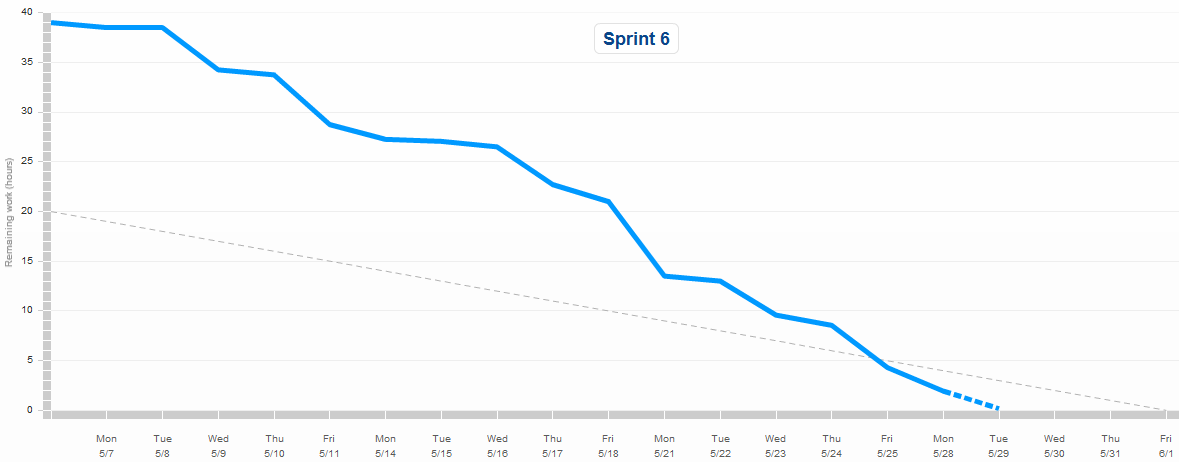
\includegraphics[scale=0.25]{Billeder/Sprint6_burn.png}
	    \vspace{-20pt}
	\caption{Burndown chart for sprint 6}
  \label{fig:sprint6}
      \vspace{-10pt}
\end{wrapfigure}
Derfor blev der brugt tid p�, at f� de sidste funktionaliteter i programmerne finpudset samtidig med, at de sidste dele blev implementeret. 
Et designproblem med databasen og dennes samspil med log-funktionaliteten udl�ste en mindre udfordring med systemet, men efter nogle diagrammer over de enkelte filers afh�ngigheder var skitseret, blev udfordringen l�st relativt gnidningsfrit. 
\\
\\
De sidste 14 dage stod prim�rt p� dokumentering af systemet. Her blev accepttesten tilrettet efter kravspecifikationen, samtidig med at processrapporten og designdokumentet for alvor blev udviklet.
\\
Der var ogs� planlagt, at der de sidste 14 dage skulle v�re et "kodestop", dvs. at alt ud\-vikling af kode skulle oph�re.
Men da nogle endelige tests blev udf�rt viste det sig, at der var mangler i programmet, s� systemet ikke overholdt accepttesten.
Der blev derfor brugt yderligere 3 dage for 2-3 mand p�, at teste koden for sm�fejl og f� disse rettet.


\end{document}